\section{United States Grand Prix}

\subsection{Circuit Analysis}

\textbf{Circuit Name:} Circuit of the Americas (Austin, Texas, USA) \\
\textbf{Length:} 5.513 km - \textbf{Laps:} 56 - \textbf{Total Distance:} 308.405 km

\begin{figure}[H]
    \centering
    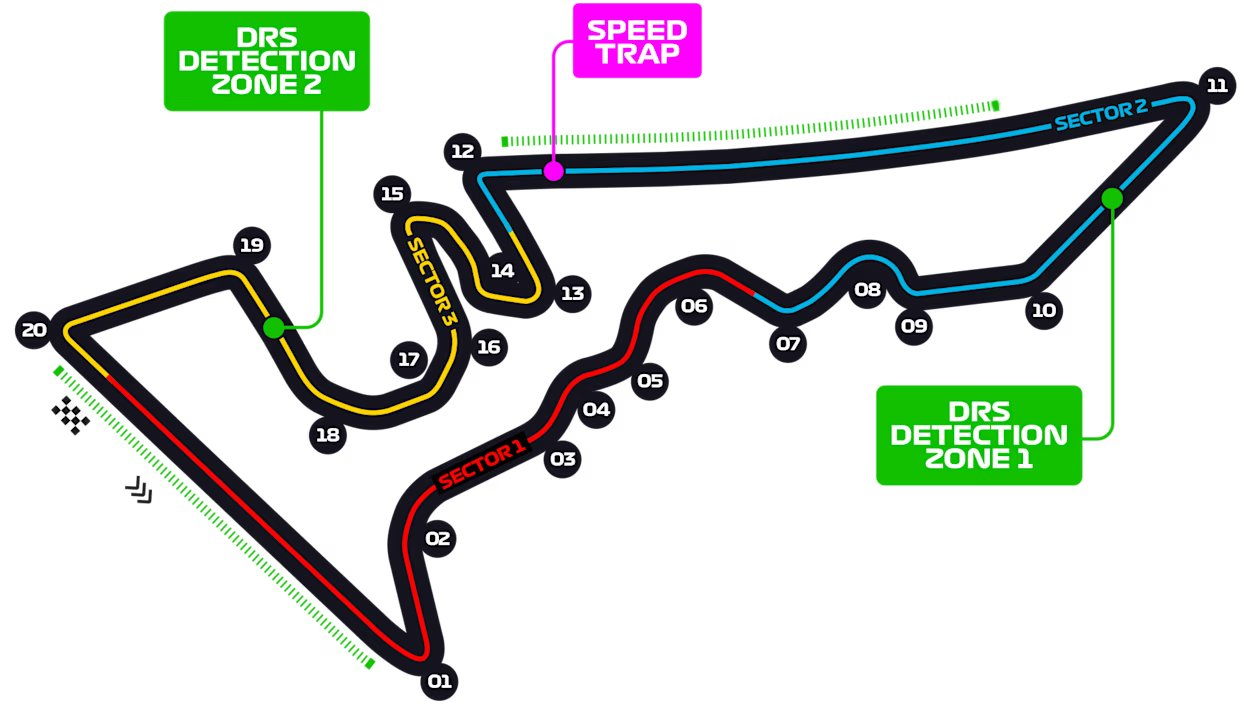
\includegraphics[width=0.75\linewidth]{images/19.United_States_Circuit.jpg}
\end{figure}

\begin{itemize}
    \item \textbf{Lap Record} : 1:32.029 (2019, Valterri Bottas – Red Bull).
    
    \item \textbf{Number of Corners \& Key Features} : 20 turns (8 right, 12 left), highly technical mix of high-speed esses, tight hairpins, and long straights. \\
    Iconic uphill run into Turn 1, wide entry allowing multiple lines. 
    
    \item \textbf{Braking Zones \& Traction} : Heavy braking at Turn 1 and Turn 12. \\
    Rear stability critical for acceleration out of slow corners.
    
    \item \textbf{DRS \& Overtaking} : Two DRS zones (main straight and back straight into Turn 12). \\
    Multiple overtaking opportunities but strong defence possible due to wide track.
    
    \item \textbf{Tyre Degradation \& Strategy} : Medium degradation, high rear wear. \\
    Undercuts very powerful due to long pit exit loss and track layout. \\
    Two-stop strategies most effective.
    
    \item \textbf{Weather \& Environment} : Warm Texan climate, bumpy asphalt. \\
    Circuit demands both aero efficiency and mechanical grip.
\end{itemize}

\textbf{Strategic Summary :} COTA rewards cars with strong straight-line speed, good traction, and ability to manage high-energy corners. Strategy is often defined by the undercut power and defending into Turn 12.

\subsection{Race Analysis}

\textbf{Date:} Sprint : 19 October 2024 - 13:00 local time\\
Race : 20 October 2024 — 14:00 local time 

\begin{itemize}
    \item \textbf{Sprint Qualifying:} \textbf{Pole Position:} Max Verstappen (Reb Bull) - 1:32.833.\\
    Grid : Russell 2nd, Leclerc 3rd, Norris 4th. \\
    Haas surprised with both cars in SQ3 (Hülkenberg P6, Magnussen P8). Piastri eliminated early (P16).
    
    \item \textbf{Sprint Race Summary:} \textbf{Winner:} Max Verstappen (Red Bull). \\
    \textbf{Podium:} 1. Verstappen - 2. Sainz - 3. Norris. \\
    Leclerc P4, Mercedes in points (Russell P5, Hamilton P6), Haas scored (Magnussen P7, Hülkenberg P8). \\
    Piastri finished outside points.
    
    \item \textbf{Qualifying Summary:} \textbf{Pole Position:} Lando Norris (McLaren) – 1:32.330. \\
    Grid : Verstappen 2nd, Sainz 3rd, Leclerc 4th. \\
    Hamilton shock Q1 elimination (P19).
    
    \item \textbf{Race Summary:} \textbf{Winner:} Charles Leclerc (Ferrari) — lights-to-flag dominance after Turn 1 move. \\
    \textbf{Podium:} 1. Leclerc - 2. Sainz - 3. Verstappen. \\
    Norris crossed P3 but penalised 5s for off-track pass, classified P4. \\
    Ferrari celebrated their second 1–2 of the season. \\
    \textbf{Notable incidents:} Hamilton crashed out lap 2. \\
    Lawson (P9) and Colapinto (P10) both scored first career points.
    
    \item \textbf{Strategies:} \\
    - Leclerc: medium → hard (lap 26), flawless execution. \\
    - Sainz: undercut Verstappen between laps 21–25, decisive for P2. \\
    - Verstappen: medium → hard, lacked pace against Ferraris, defended hard vs Norris. \\
    - Norris: extended first stint (lap 31), tried fresher tyres late, penalised for pass. \\
    - Piastri: steady but stuck behind top 4, finished P5. \\
    - Russell: pitlane start + penalty, recovered to P6. \\
    - Ocon: fastest lap on softs but outside top 10, no bonus point.
    
    \item \textbf{Performance Trends:} \textbf{Ferrari} strongest race pace all season, clear 1–2. \\
    \textbf{Red Bull} fast in sprint but weaker in GP, Verstappen forced into defence. \\
    \textbf{McLaren} strong on Saturday but race execution compromised by penalties. \\
    \textbf{Mercedes} mixed: Russell recovered, Hamilton eliminated early. \\
    \textbf{Haas} consistent points, \textbf{Williams} breakthrough with Colapinto, Lawson scored on \textbf{Racing Bulls} debut.
    
    \item \textbf{Championship Impact:} \textbf{Drivers:} Verstappen 354 pts, Norris 297, Leclerc 275. \\
    \textbf{Constructors:} McLaren 544, Red Bull 504, Ferrari 496, Mercedes 344.
\end{itemize}

\textbf{Key Takeaway :} Ferrari delivered a dominant 1–2, with Leclerc in control from Turn 1 and Sainz executing the decisive undercut on Verstappen. McLaren showed raw pace but faltered in race execution, while Red Bull had no answer to Ferrari’s superior tyre life.

\subsection{Link \& Takeaway}

\begin{itemize}
    \item COTA’s wide layout and heavy braking zones favoured Ferrari’s strong traction and straight-line speed. Leclerc’s Turn 1 move set the tone for the race. 
    \item Sainz capitalised on undercut power at Austin to secure Ferrari’s 1–2, showing the team’s sharp race management. 
    \item Verstappen salvaged podiums across sprint and race but showed Red Bull’s vulnerability in tyre longevity compared to Ferrari. 
    \item Norris’ penalty underlined how strict track limits at COTA can reshape results, even in late-race battles. 
    \item Lawson and Colapinto’s points showed how unpredictable COTA can be for midfield teams, with opportunities emerging from attrition and penalties. 
    \item Ferrari’s dominant pace gave them their biggest points haul of the season, reigniting their constructors’ title hopes.
\end{itemize}
